\documentclass[12pt,letterpaper]{article}

% ===================== PAQUETES =====================
\usepackage[utf8]{inputenc}
\usepackage[T1]{fontenc}
\usepackage{graphicx}
\usepackage{float}
\usepackage{listings}
\usepackage{xcolor}
\usepackage{hyperref}
\usepackage{geometry}
\usepackage{amsmath}
\usepackage{booktabs}
\usepackage{array}

% NOTA: el paquete babel con soporte de idioma espanol (spanish.ldf) no esta
% disponible en este entorno de compilacion, por lo que se omite \usepackage{babel}.
% Esto no afecta el contenido del informe, que esta redactado integramente en
% espanol; unicamente implica que textos automaticos de LaTeX (indices, etc.,
% que no se usan en este documento) permanecerian en ingles si se utilizaran.
\renewcommand{\contentsname}{Índice}
\renewcommand{\figurename}{Figura}
\renewcommand{\tablename}{Tabla}

% ===================== MARGENES =====================
\geometry{margin=2.5cm}

% ===================== ESTILO DE CODIGO =====================
\definecolor{colorFondoCodigo}{rgb}{0.97,0.97,0.97}
\definecolor{colorComentario}{rgb}{0.0,0.5,0.0}
\definecolor{colorPalabraClave}{rgb}{0.0,0.0,0.7}
\definecolor{colorCadena}{rgb}{0.6,0.0,0.0}

\lstdefinestyle{estiloC}{
    backgroundcolor=\color{colorFondoCodigo},
    commentstyle=\color{colorComentario},
    keywordstyle=\color{colorPalabraClave}\bfseries,
    stringstyle=\color{colorCadena},
    basicstyle=\footnotesize\ttfamily,
    breakatwhitespace=false,
    breaklines=true,
    captionpos=b,
    keepspaces=true,
    numbers=left,
    numbersep=5pt,
    numberstyle=\tiny\color{gray},
    showspaces=false,
    showstringspaces=false,
    showtabs=false,
    tabsize=2,
    frame=single,
    language=C
}
\lstset{style=estiloC}

% ===================== HYPERREF =====================
\hypersetup{
    colorlinks=true,
    linkcolor=blue,
    urlcolor=blue,
    citecolor=blue,
    pdftitle={Evaluacion 3 Unidad 3: Arboles y Grafos},
    pdfauthor={Estudiantes INF-213}
}

\title{
    \textbf{Evaluación 3 Unidad 3: Árboles y Grafos} \\[0.3cm]
    \large INF-213 Estructura de Datos
}
\author{
    Rubén Sánchez \\
    Diego Solís \\
    Benjamín Vásquez \\
    Joaquín Vásquez
}
\date{
    Académico: PhD (c) Nicolás A. Reyes-Reyes \\[0.2cm]
    Fecha de entrega: 31 de junio de 2026
}

\begin{document}

\maketitle
\thispagestyle{empty}
\newpage

\setcounter{page}{1}

\section{Introducción}

Los grafos son una de las estructuras de datos no lineales más utilizadas para modelar
problemas del mundo real en los que existen elementos interconectados, como redes de
transporte, redes eléctricas o sistemas de rutas urbanas. A través de un grafo es posible
representar tanto la posición de cada elemento (nodo) como el costo o distancia asociado a
desplazarse entre ellos (arista), lo que permite aplicar algoritmos clásicos de optimización
para resolver problemas concretos de conectividad y de recorrido. En este informe se aborda,
por un lado, el problema del árbol de expansión mínima (MST) sobre un conjunto de 25 puntos de
interés reales de la ciudad de Talca, comparando tres algoritmos distintos (Prim, Kruskal y
Borůvka); y por otro lado, el problema del vendedor viajero (TSP) aplicado al diseño de un
recorrido de bus de acercamiento de la Universidad Católica del Maule, resuelto mediante la
metaheurística GRASP. El objetivo central es aplicar los TADs de grafos, conjuntos disjuntos y
colas de prioridad estudiados en la asignatura, evaluando su correctitud y eficiencia frente a
instancias de tamaño realista. Este tipo de problemas tiene una importancia práctica directa en
el transporte y la logística, donde minimizar distancias recorridas se traduce en ahorros de
tiempo, combustible y en la posibilidad de aumentar la frecuencia de los servicios ofrecidos.

\section{Ejercicio 1: Árbol de Expansión Mínima}

\subsection{Modelado del problema}

Para este ejercicio se seleccionó la ciudad de Talca, Región del Maule, debido a la buena
disponibilidad de información geográfica de sus puntos de interés en Google Maps. Se
identificaron 25 puntos de interés representativos de distintos sectores de la ciudad: plazas,
universidades, hospitales, museos, centros comerciales, estaciones de transporte y zonas
periféricas, entre otros. Cada punto de interés se modeló como un nodo del TAD \texttt{Grafo},
almacenando su nombre y sus coordenadas geográficas (latitud y longitud).

El grafo se construyó como un grafo no dirigido y completo: se agregó una arista entre cada par
posible de los 25 nodos, lo que da un total de $\binom{25}{2} = 300$ aristas. El peso de cada
arista se calculó mediante la función \texttt{distancia\_euclidiana\_aprox}, que aplica una
proyección equirectangular sobre las coordenadas geográficas, corrigiendo la diferencia de
longitud por el coseno de la latitud promedio entre ambos puntos y escalando el resultado por el
radio de la Tierra (6.372,8 km). Esta aproximación es adecuada dado que todos los puntos de
interés se encuentran a distancias relativamente pequeñas entre sí (dentro de la misma ciudad).
Toda esta información se almacena en una matriz de adyacencia de $25\times25$, que se imprime
completa como parte de la salida del programa.

\subsection{Algoritmos implementados}

Se implementaron tres algoritmos distintos para obtener el árbol de expansión mínima (MST) del
grafo construido:

\begin{itemize}
    \item \textbf{Prim}: parte de un nodo inicial y hace crecer un único árbol agregando, en
    cada paso, la arista de menor peso que conecta el árbol actual con un nodo todavía no
    incluido. Para encontrar eficientemente esa arista mínima se utilizó el TAD
    \texttt{MinHeap} (cola de prioridad implementada como heap binario en arreglo), que permite
    extraer el nodo de menor prioridad y disminuir prioridades en tiempo logarítmico.

    \item \textbf{Kruskal}: ordena todas las aristas del grafo de menor a mayor peso (usando
    \texttt{qsort}) y las recorre en ese orden, agregando cada una al MST solo si sus extremos no
    pertenecen todavía al mismo componente conexo, lo que se verifica mediante el TAD
    \texttt{ConjuntosDisjuntos} (Union-Find) con las optimizaciones de compresión de camino y
    unión por rango.

    \item \textbf{Borůvka}: a diferencia de los anteriores, trabaja por rondas. En cada ronda,
    cada componente conexo busca la arista más barata que lo conecta con un componente distinto,
    y todas esas aristas "ganadoras" se agregan simultáneamente, también apoyándose en
    \texttt{ConjuntosDisjuntos}. El número de componentes se reduce significativamente en cada
    ronda, por lo que el algoritmo converge en $O(\log N)$ rondas.
\end{itemize}

\subsection{Pruebas de ejecución}

\subsubsection*{Prueba 1: comparación de los tres algoritmos}

Se ejecutaron los tres algoritmos sobre el mismo grafo de 25 nodos, partiendo Prim desde el nodo
0 (Plaza de Armas). Los resultados obtenidos en la ejecución real del programa fueron:

\begin{table}[H]
\centering
\begin{tabular}{lc}
\toprule
\textbf{Algoritmo} & \textbf{Peso total del MST (km)} \\
\midrule
Prim    & 21.7309 \\
Kruskal & 21.7309 \\
Borůvka & 21.7309 \\
\bottomrule
\end{tabular}
\caption{Comparación de pesos totales obtenidos por los tres algoritmos de MST.}
\end{table}

Los tres algoritmos obtuvieron exactamente el mismo árbol de expansión mínima, con un peso
total de 21,7309 km y 24 aristas (es decir, $N-1$ aristas para $N=25$ nodos), consistente con la
definición de árbol de expansión. Algunas de las aristas más cortas encontradas corresponden a
puntos cercanos del centro histórico, como Plaza de Armas -- Centro Histórico (0,0929 km) o
Centro Histórico -- Museo O'Brien (0,0859 km), mientras que la arista más costosa del árbol
conecta sectores periféricos, como Villa Cultural Huilquilemu -- Camino a San Clemente
(5,4124 km).

\begin{figure}[H]
\centering
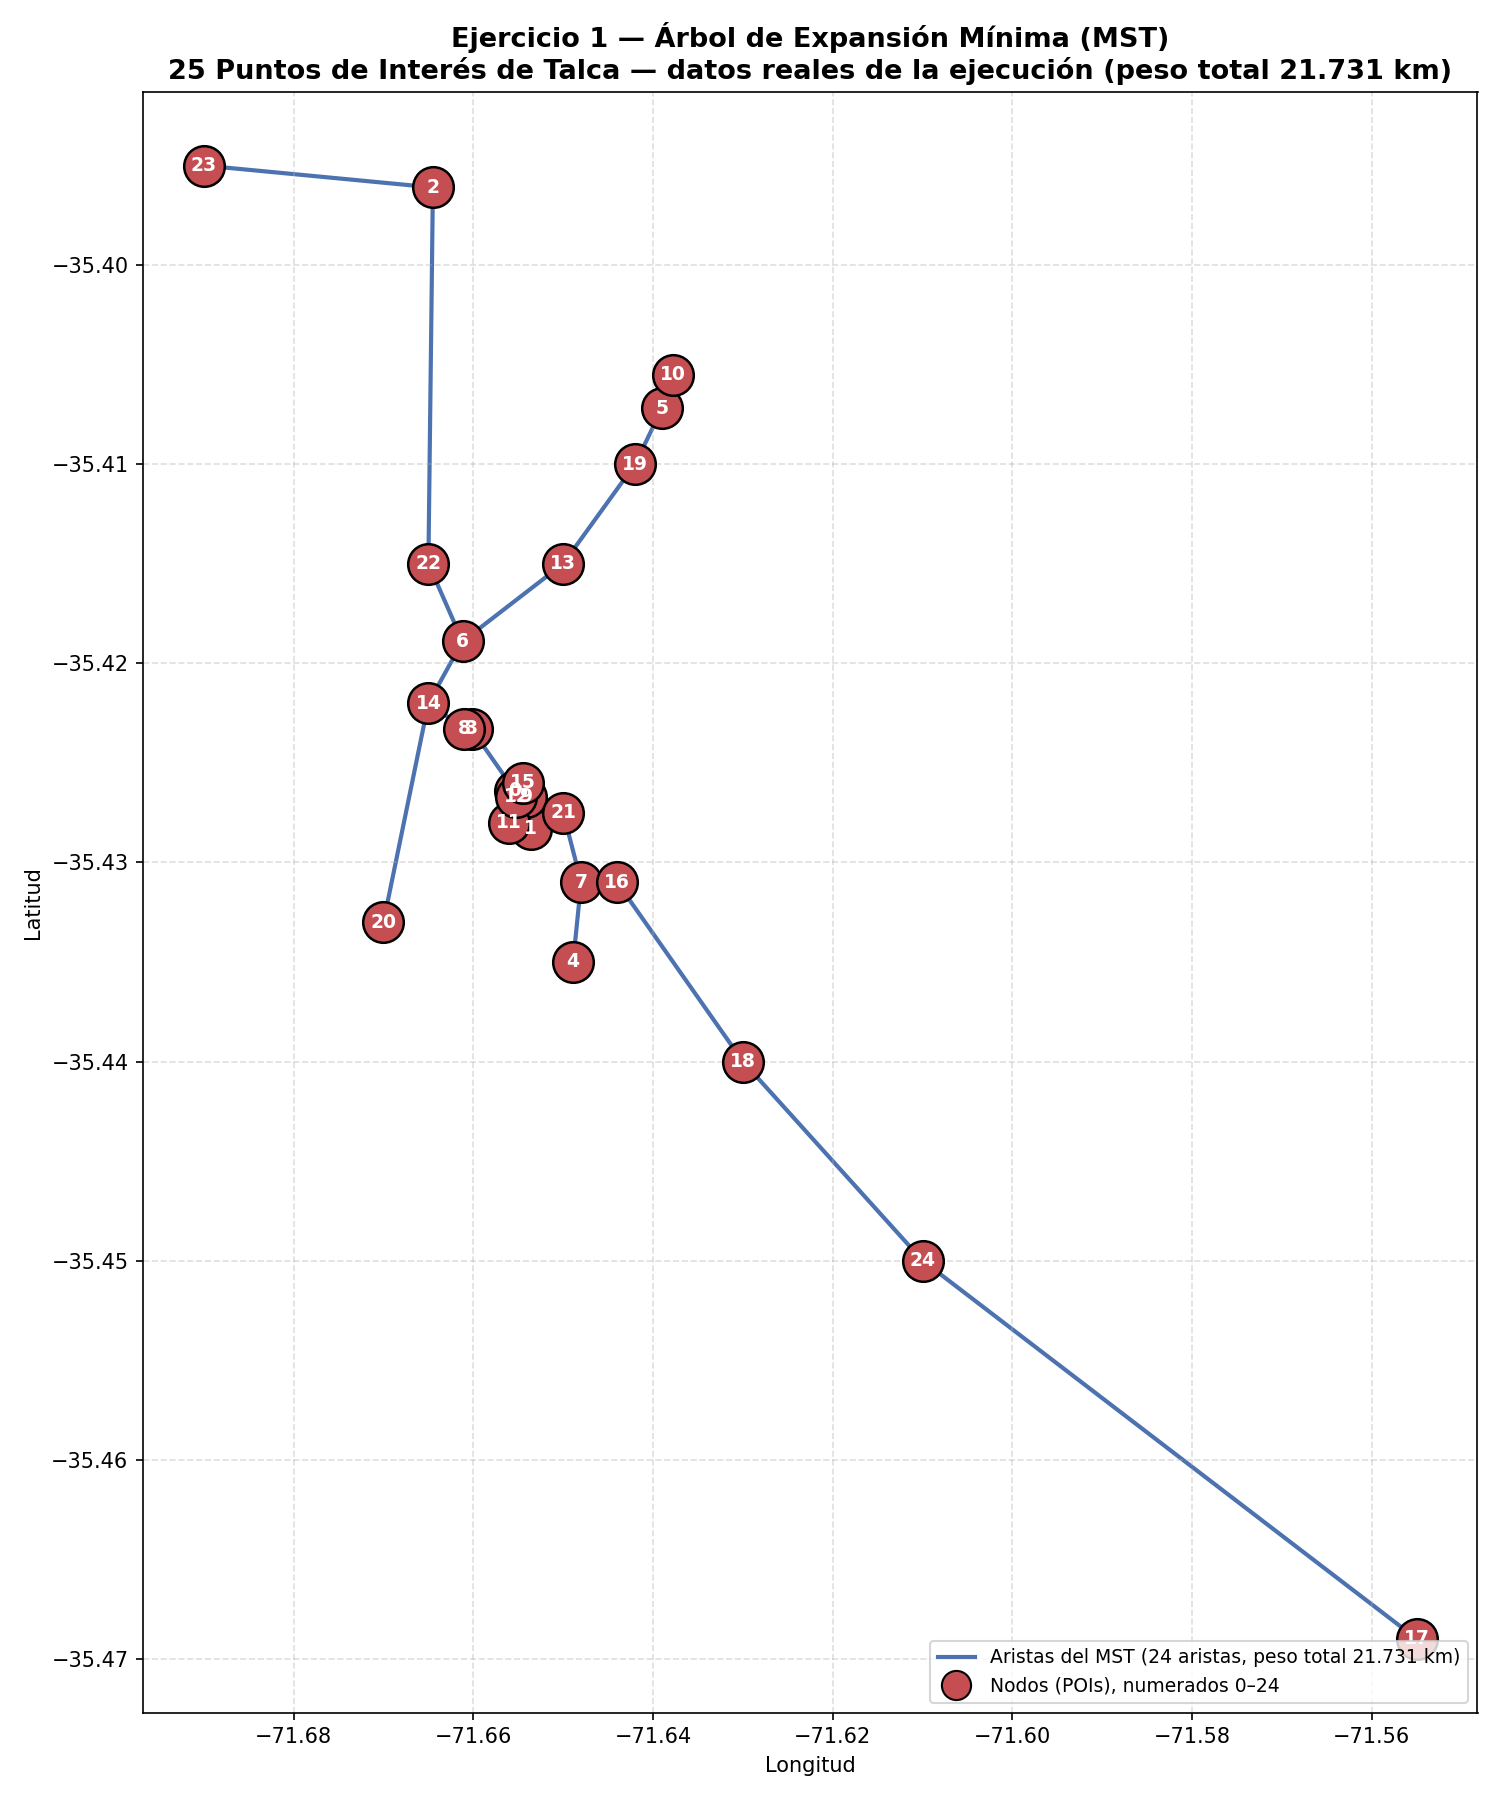
\includegraphics[width=0.85\textwidth]{ejercicio1_mst.png}
\caption{Árbol de expansión mínima obtenido sobre los 25 puntos de interés de Talca. Las
coordenadas y las 24 aristas mostradas corresponden exactamente a la salida real del programa
(archivo \texttt{resultado\_ejercicio1.txt}); el peso total coincide con el reportado por los
tres algoritmos (21,7309 km).}
\end{figure}

\subsubsection*{Prueba 2: Prim desde distintos nodos iniciales}

Para verificar que el peso total del MST no depende del nodo desde el cual se inicia la
construcción, se ejecutó el algoritmo de Prim partiendo desde tres nodos distintos: el nodo 0
(Plaza de Armas), el nodo 5 (Mall Plaza Maule) y el nodo 12 (Catedral de Talca).

\begin{table}[H]
\centering
\begin{tabular}{lc}
\toprule
\textbf{Nodo inicial} & \textbf{Peso total del MST (km)} \\
\midrule
0  -- Plaza de Armas     & 21.7309 \\
5  -- Mall Plaza Maule   & 21.7309 \\
12 -- Catedral de Talca  & 21.7309 \\
\bottomrule
\end{tabular}
\caption{Peso total del MST obtenido con Prim desde distintos nodos de inicio.}
\end{table}

La diferencia máxima entre los tres resultados fue de 0,000000 km, confirmando que el peso del
MST es independiente del nodo de inicio elegido.

\subsection{Análisis}

Los resultados obtenidos confirman lo que predice la teoría de grafos: cuando un grafo es conexo
y ponderado, el árbol de expansión mínima es único en cuanto a su peso total (aunque puede
existir más de un conjunto de aristas que alcance ese mismo peso mínimo cuando hay pesos
repetidos o muy similares entre sí). Los tres algoritmos implementados --Prim, Kruskal y
Borůvka-- parten de estrategias distintas (crecimiento de un único árbol, orden global de
aristas, y fusión de componentes por rondas, respectivamente), pero al ser todos correctos
desde el punto de vista de la teoría de optimización combinatoria, convergen al mismo resultado
óptimo. La Prueba 2 refuerza esta conclusión desde otro ángulo: independientemente de cuál sea
el nodo de partida, Prim siempre encuentra un árbol del mismo peso total, ya que el algoritmo
garantiza optimalidad sin importar el punto de inicio, cambiando únicamente la forma en que se
recorre el árbol pero no su costo final.

\section{Ejercicio 2: Problema del Vendedor Viajero (TSP)}

\subsection{Modelado del problema}

Para este ejercicio se modeló el recorrido del bus de acercamiento de la Universidad Católica
del Maule (UCM) en la ciudad de Talca. Se definieron 5 zonas de la ciudad --Centro, Sur, Norte,
Oriente y Poniente--, y dentro de cada zona se escogieron 10 ubicaciones reales (50 ubicaciones
en total), correspondientes a lugares como universidades, parques, colegios, centros de salud y
plazas de cada sector. La primera ubicación registrada en la zona Centro corresponde
precisamente a la UCM, siendo el nodo de id 0 dentro del grafo.

Las ubicaciones dentro de cada zona se conectaron de forma completa (subgrafo $K_{10}$): cada
una de las 10 ubicaciones de una zona es adyacente directamente a las otras 9 de la misma zona.
Adicionalmente, se agregaron 5 conexiones entre ubicaciones de zonas distintas, enlazando
sectores vecinos a través de puntos geográficamente cercanos entre ellos. Todas las distancias,
tanto dentro de una zona como entre zonas distintas, se calcularon mediante la fórmula del
\textbf{haversine}, que considera la curvatura de la Tierra y resulta más precisa que una
aproximación euclidiana para este tipo de análisis de rutas.

Como el grafo resultante no es completo (solo existe conexión total dentro de cada zona y un
número reducido de aristas entre zonas), no es posible conocer de antemano la distancia más
corta entre dos ubicaciones de zonas distintas que no estén directamente conectadas. Por este
motivo se aplicó el algoritmo de \textbf{Floyd-Warshall}, que calcula la distancia del camino
más corto entre todos los pares de nodos del grafo, considerando los posibles caminos a través
de nodos intermedios. Esta matriz de distancias mínimas es la que efectivamente utiliza GRASP
para evaluar y comparar los distintos circuitos candidatos.

\subsection{Algoritmo GRASP}

GRASP (\textit{Greedy Randomized Adaptive Search Procedure}, o "Procedimiento de Búsqueda Voraz
Adaptativo Aleatorizado") es una metaheurística que combina, en cada iteración, una fase de
construcción voraz aleatorizada con una fase de búsqueda local, repitiendo este ciclo muchas
veces para obtener una buena aproximación a la solución óptima.

\textbf{Fase de construcción con RCL.} En cada paso de la construcción del circuito, en lugar de
elegir siempre el nodo no visitado más cercano (estrategia puramente voraz), se construye una
\textit{Lista de Candidatos Restringida} (RCL) que incluye a todos los nodos no visitados cuya
distancia al último nodo agregado se encuentre dentro de un umbral. Dicho umbral se calcula como
$\text{umbral} = d_{\min} + \alpha \cdot (d_{\max} - d_{\min})$, donde $d_{\min}$ y $d_{\max}$
son, respectivamente, la menor y la mayor distancia entre el nodo actual y los nodos aún no
visitados. Finalmente, se elige aleatoriamente uno de los nodos de la RCL para continuar el
circuito. El parámetro $\alpha \in [0,1]$ controla el balance entre \textit{explotación} y
\textit{exploración}: con $\alpha = 0$, solo el nodo más cercano puede entrar a la RCL
(comportamiento voraz puro); con $\alpha = 1$, todos los nodos no visitados entran a la RCL
(selección esencialmente aleatoria).

\textbf{Búsqueda local 2-opt.} Una vez construido un circuito completo, se aplica el movimiento
2-opt: se prueban pares de aristas del circuito y se evalúa si invertir el segmento de ruta entre
ellas reduce la distancia total. El nodo de inicio (la UCM) se mantiene siempre fijo en su
posición, ya que el recorrido debe comenzar y terminar en ese punto. El proceso se repite hasta
que ninguna inversión adicional logra mejorar el circuito, alcanzando así un óptimo local.

\subsection{Pruebas de ejecución}

\subsubsection*{Prueba 1: GRASP con $\alpha = 0{,}3$ y 200 iteraciones}

Se ejecutó GRASP con $\alpha = 0{,}3$ durante 200 iteraciones sobre el grafo de 50 ubicaciones.
El mejor circuito encontrado por el programa obtuvo una distancia total de \textbf{56,2558 km},
visitando las 50 ubicaciones de las 5 zonas y retornando finalmente a la UCM. El recorrido
agrupa de forma natural las ubicaciones cercanas entre sí (dentro de una misma zona) antes de
desplazarse hacia la siguiente zona, lo cual es coherente con la estructura del grafo, donde las
conexiones intra-zona son mucho más numerosas que las conexiones inter-zona.

\begin{figure}[H]
\centering
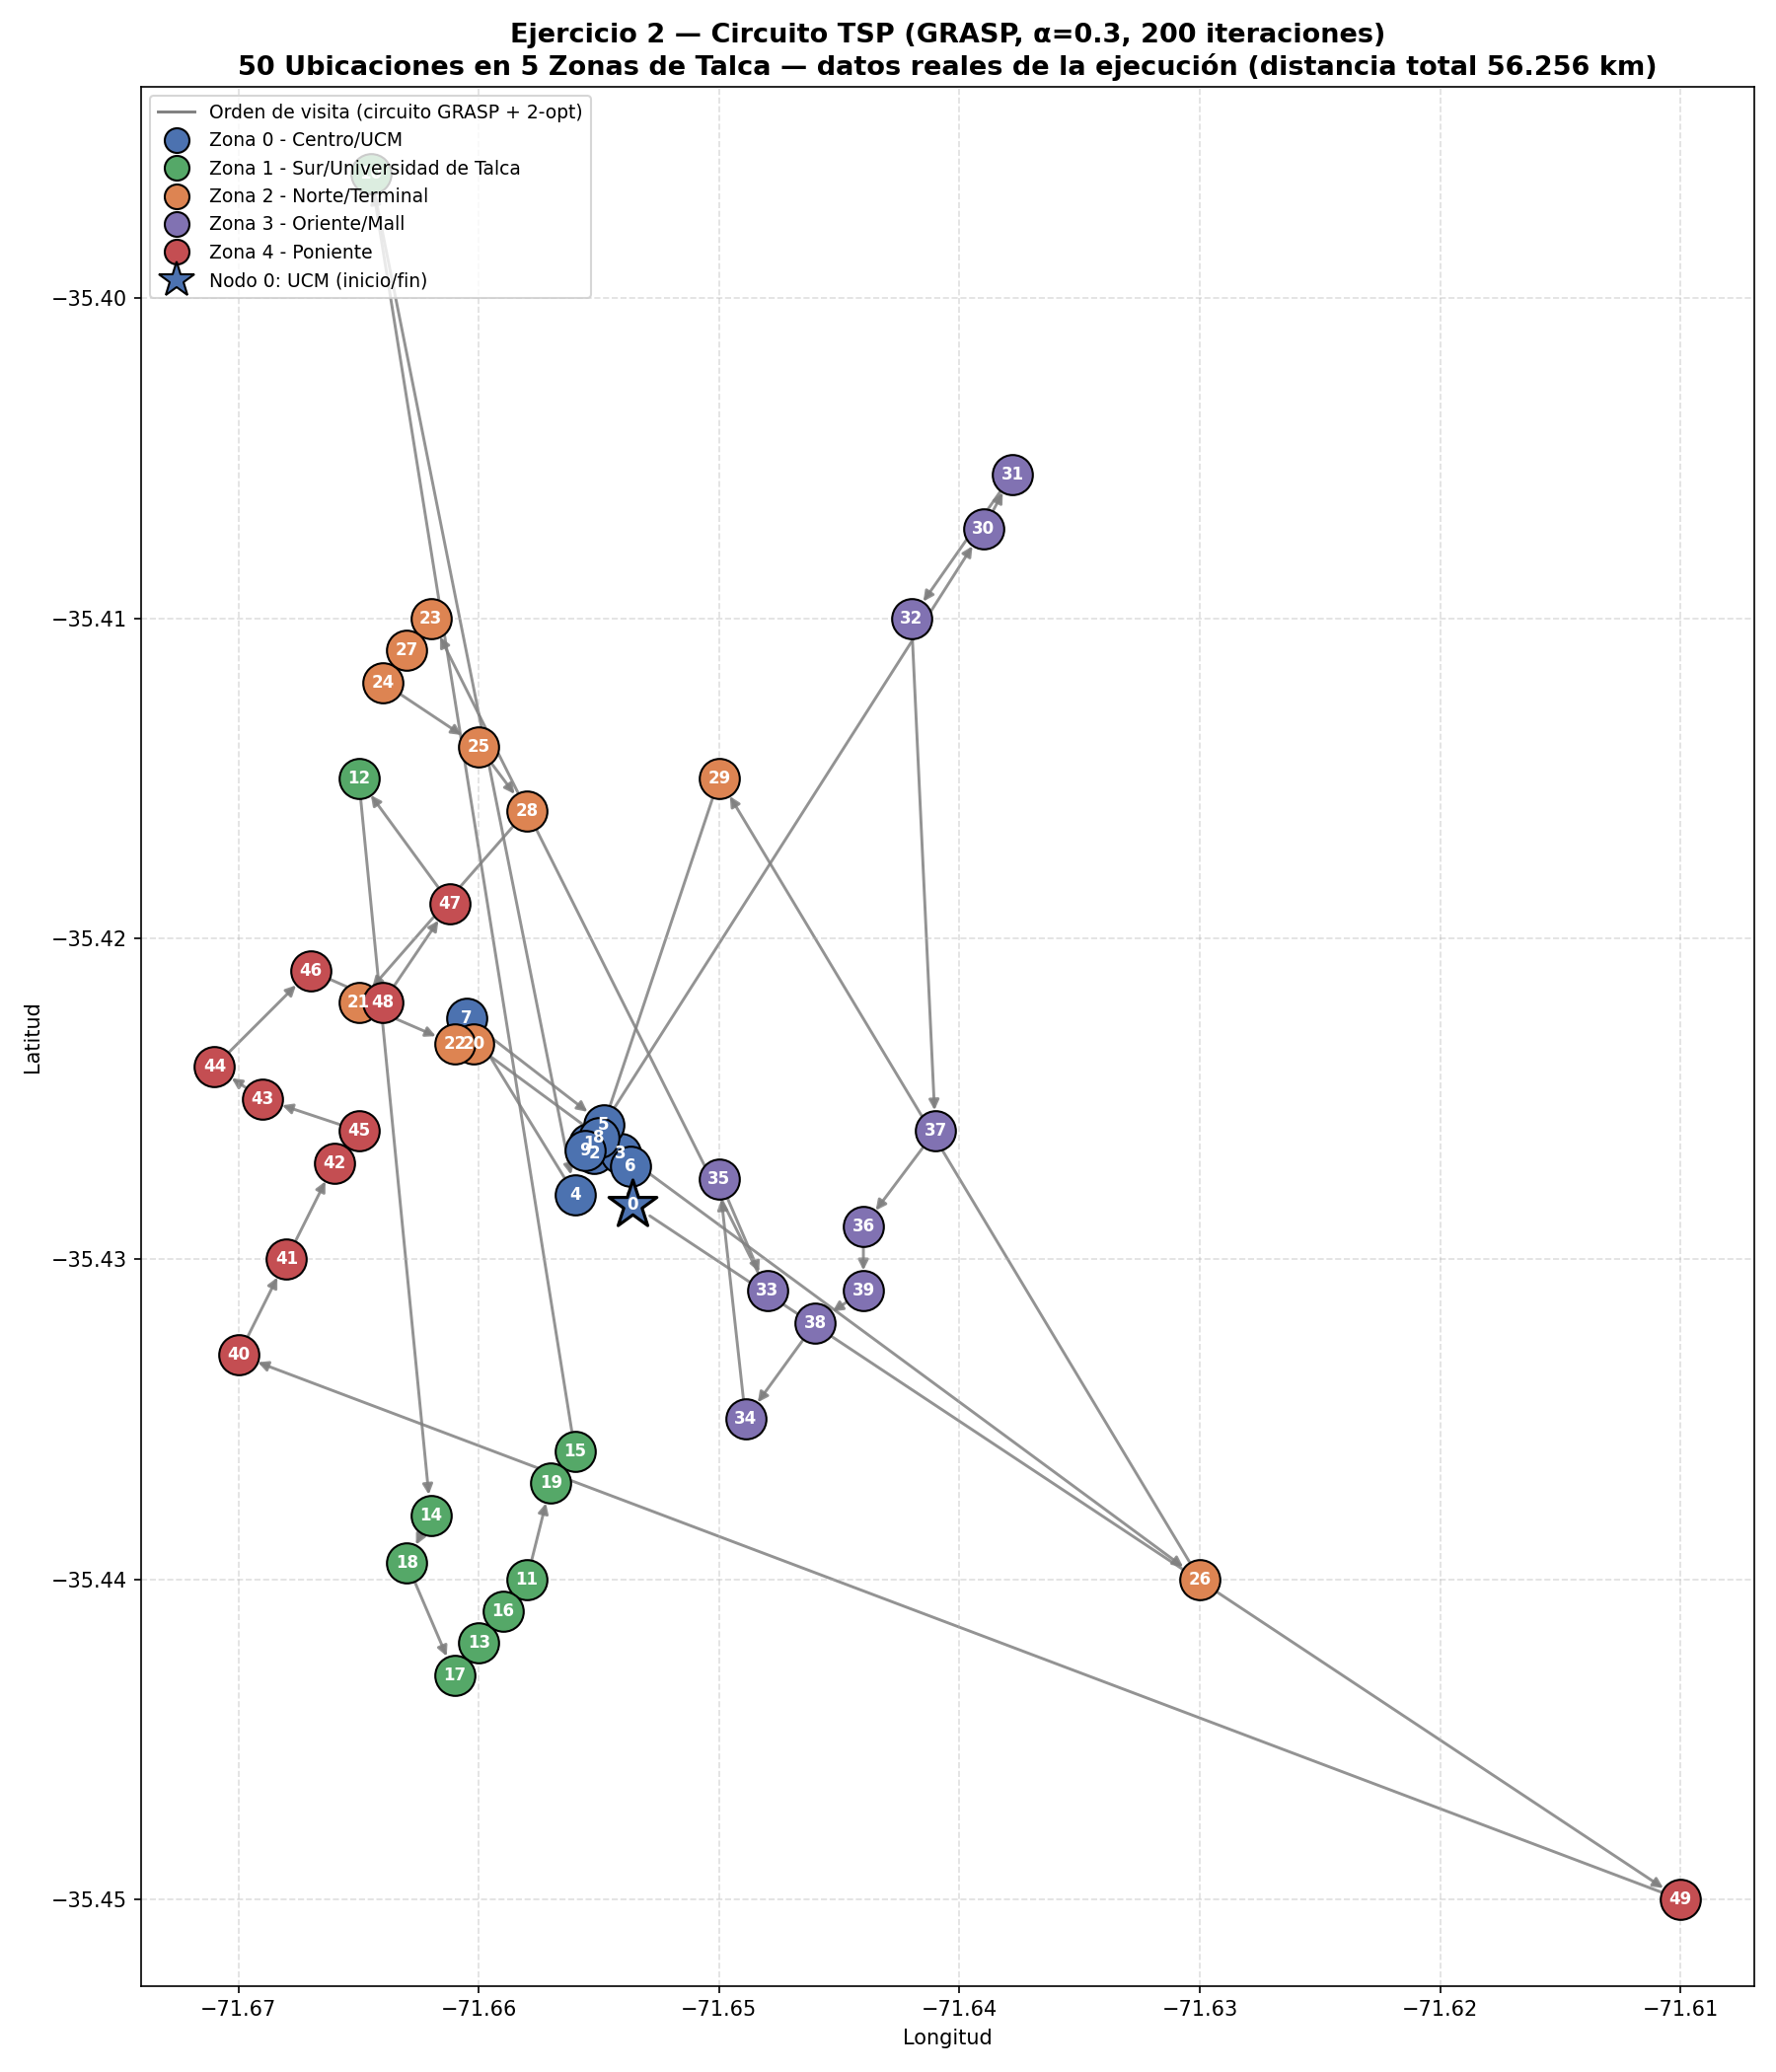
\includegraphics[width=0.9\textwidth]{ejercicio2_tsp.png}
\caption{Circuito TSP obtenido por GRASP ($\alpha=0{,}3$, 200 iteraciones) sobre las 50
ubicaciones de las 5 zonas de Talca. Las flechas indican el orden exacto de visita reportado por
el programa (archivo \texttt{resultado\_ejercicio2.txt}); el nodo 0 (estrella) corresponde a la
UCM, punto de inicio y de retorno del circuito. La distancia total (56,2558 km) coincide con la
reportada en la ejecución real.}
\end{figure}

\subsubsection*{Prueba 2: comparación de distintos valores de alpha}

Se ejecutó GRASP con cuatro valores distintos de $\alpha$ (0,0, 0,3, 0,7 y 1,0), cada uno con 200
iteraciones, obteniendo los siguientes resultados:

\begin{table}[H]
\centering
\begin{tabular}{cc}
\toprule
\textbf{Valor de $\alpha$} & \textbf{Distancia total (km)} \\
\midrule
0,0 & 57,2978 \\
0,3 & 56,2558 \\
0,7 & 56,2558 \\
1,0 & 56,2558 \\
\bottomrule
\end{tabular}
\caption{Distancia total del mejor circuito GRASP para distintos valores de $\alpha$ (200 iteraciones cada uno).}
\end{table}

\subsection{Análisis y recomendación}

A diferencia de lo que suele esperarse de forma intuitiva --que un comportamiento totalmente
voraz ($\alpha = 0$) entregue siempre el mejor resultado--, en esta instancia particular del
problema se observó el efecto contrario: $\alpha = 0$ obtuvo la \emph{peor} distancia total
(57,2978 km), mientras que $\alpha = 0{,}3$, $0{,}7$ y $1{,}0$ convergieron de manera consistente
a un resultado mejor (56,2558 km). Este comportamiento, lejos de ser un error, ilustra una
propiedad importante de las metaheurísticas tipo GRASP: cuando $\alpha = 0$, la RCL contiene
prácticamente un único candidato en cada paso, por lo que la fase de construcción se vuelve
\emph{determinista}. Esto significa que las 200 iteraciones generan exactamente el mismo
circuito inicial, y la búsqueda local 2-opt dispone de un solo punto de partida desde el cual
intentar mejorar la solución, quedando atrapada en su óptimo local correspondiente. En cambio,
con $\alpha > 0$ cada iteración construye un circuito inicial distinto, lo que le da a la fase de
búsqueda local múltiples puntos de partida diferentes desde los cuales explorar el espacio de
soluciones, aumentando la probabilidad de escapar de óptimos locales mediocres y de encontrar un
circuito de menor distancia total.

Para el caso del bus de acercamiento de la UCM, esta observación tiene una implicancia práctica
relevante: no conviene utilizar GRASP en su variante completamente voraz, ya que pierde la
capacidad exploratoria que es justamente la fuente de su buen desempeño práctico frente a una
heurística voraz simple. Se recomienda utilizar un valor de $\alpha$ moderado (en torno a
$0{,}3$), que mantiene una construcción mayoritariamente guiada por la cercanía geográfica --
favoreciendo rutas razonables y evitando saltos excesivos entre ubicaciones lejanas-- pero
conservando suficiente diversidad entre iteraciones para que la búsqueda local 2-opt pueda
explorar distintos óptimos locales y converger a una solución de buena calidad, tal como lo
muestran los resultados obtenidos en las pruebas de ejecución.

\section{Conclusiones}

El desarrollo de esta evaluación permitió aplicar de manera práctica los TADs de estructuras no
lineales estudiados en el curso --grafos, conjuntos disjuntos y colas de prioridad-- sobre
problemas con datos geográficos reales. La implementación de Prim, Kruskal y Borůvka evidenció
que, aunque cada algoritmo recorre el espacio de soluciones de una forma distinta, todos son
capaces de alcanzar el árbol de expansión mínimo óptimo cuando el grafo es conexo, reforzando la
importancia de elegir la estructura auxiliar adecuada (heap para Prim, conjuntos disjuntos para
Kruskal y Borůvka) según las necesidades de cada algoritmo. Por su parte, la resolución del TSP
mediante GRASP mostró que la recursividad y las estructuras de datos eficientes no bastan por sí
solas para resolver problemas NP-difíciles de gran escala, y que metaheurísticas que combinan
aleatoriedad controlada con búsqueda local pueden encontrar soluciones de buena calidad en tiempos
razonables. En conjunto, este trabajo deja en evidencia que la elección de la estructura de datos
y del algoritmo correcto no es una decisión menor, sino que determina directamente la
correctitud, eficiencia y calidad de la solución obtenida frente a problemas de optimización que
surgen habitualmente en contextos reales de transporte y logística urbana.

\section{Anexo}

El código fuente completo que resuelve ambos ejercicios se adjunta como un archivo comprimido
(\texttt{proyecto\_grafos.zip}) junto con este informe, siguiendo la estructura de proyecto del
IDE CLion. El proyecto incluye los siguientes
módulos principales:

\begin{itemize}
    \item \texttt{salida.h / salida.c}: impresión simultánea en consola y archivo.
    \item \texttt{arbol.h / arbol.c}: TAD de conjuntos disjuntos (Union-Find).
    \item \texttt{arbol\_binario.h / arbol\_binario.c}: TAD min-heap (cola de prioridad).
    \item \texttt{distancias.h / distancias.c}: cálculo de distancias geográficas (euclidiana
    aproximada y haversine).
    \item \texttt{grafo.h / grafo.c}: TAD grafo no dirigido y ponderado, mediante matriz de
    adyacencia.
    \item \texttt{caminos\_minimos.h / caminos\_minimos.c}: algoritmo de Floyd-Warshall.
    \item \texttt{grasp\_tsp.h / grasp\_tsp.c}: algoritmo GRASP (RCL + búsqueda local 2-opt).
    \item \texttt{mst.h / mst.c}: algoritmos de Prim, Kruskal y Borůvka.
    \item \texttt{main\_ejercicio1.c} y \texttt{main\_ejercicio2.c}: programas principales de
    cada ejercicio.
\end{itemize}

A continuación se muestra, a modo de referencia, un fragmento del TAD de conjuntos disjuntos
utilizado tanto por Kruskal como por Borůvka:

\begin{lstlisting}[caption={Fragmento de arbol.c: union por rango con compresion de camino}]
int cd_encontrar(ConjuntosDisjuntos *cd, int x) {
    if (cd->padre[x] == x) {
        return x;
    }
    /* Compresion de camino: x apunta directamente a la raiz */
    cd->padre[x] = cd_encontrar(cd, cd->padre[x]);
    return cd->padre[x];
}

void cd_unir(ConjuntosDisjuntos *cd, int x, int y) {
    int raiz_x = cd_encontrar(cd, x);
    int raiz_y = cd_encontrar(cd, y);

    if (raiz_x == raiz_y) {
        return; /* Ya pertenecen al mismo conjunto */
    }
    if (cd->rango[raiz_x] < cd->rango[raiz_y]) {
        cd->padre[raiz_x] = raiz_y;
    } else if (cd->rango[raiz_x] > cd->rango[raiz_y]) {
        cd->padre[raiz_y] = raiz_x;
    } else {
        cd->padre[raiz_y] = raiz_x;
        cd->rango[raiz_x]++;
    }
}
\end{lstlisting}

\end{document}
